\newpage
\chapter{Index}
In this chapter an explanation of the index page (front page)  and the different thought and actions taken with it will be described.  
\section{Design Ideas}
The website is primarily to be used by a non-technical person at AU-Herning. The design has been kept clean to make it very intuitive how to navigate around. Periodically the energy system (and thereby also the website) is shown for high-schools students visiting the school, therefore the index page has been build up with mostly icons instead of text and a navigation bar which some of them might know from OS X (from Apple). The customer wanted the production shown as primitive things like: lightbulbs, refrigerators, money (possibly shown as number of SU payments), instead of technical terms like Joule, kW, kWh etc.
\section{The Design}

\begin{wrapfigure}{r}{0.6\textwidth}
	\center
		\setlength\fboxsep{0pt}
		\setlength\fboxrule{1pt}
		\fbox{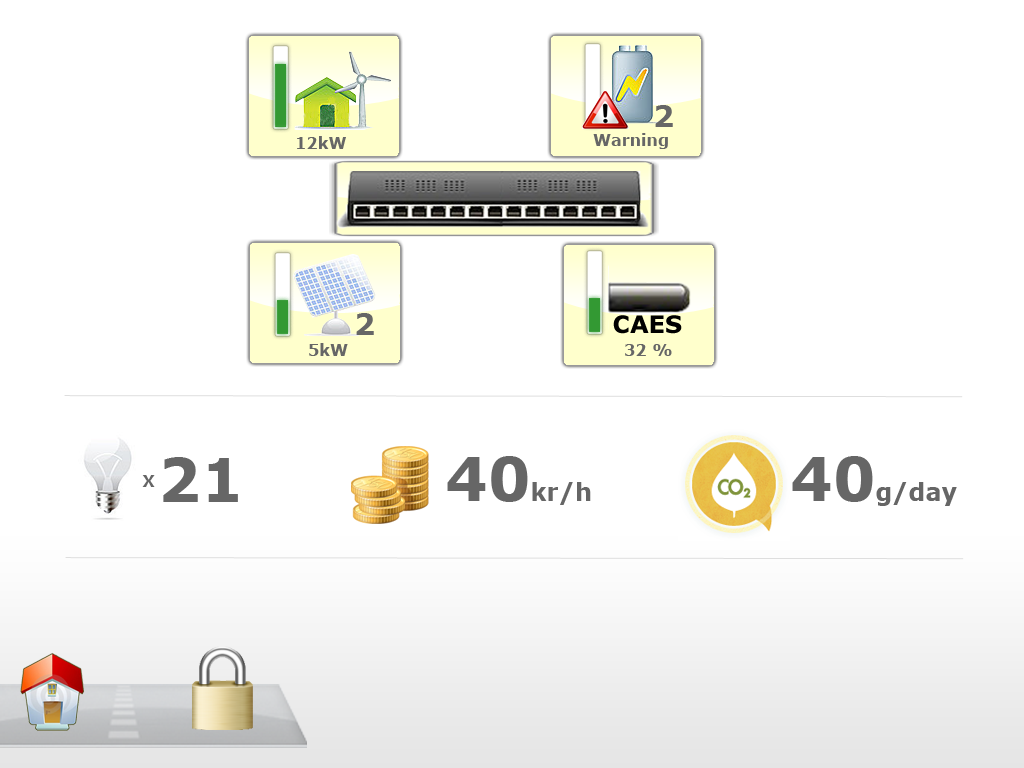
\includegraphics[width=0.6\textwidth]{images/index_design.png}}
   	\caption{First drawings of the index page.}
   	\label{fig:index_page_design}
\end{wrapfigure}
fdsa fdsa fdsa
\section{Code layout}

\section{Code explanation}

\subsection{CCS}

\subsection{HTML}